\chapter{Introduction}

\begin{figure}[h!]
    \centering
    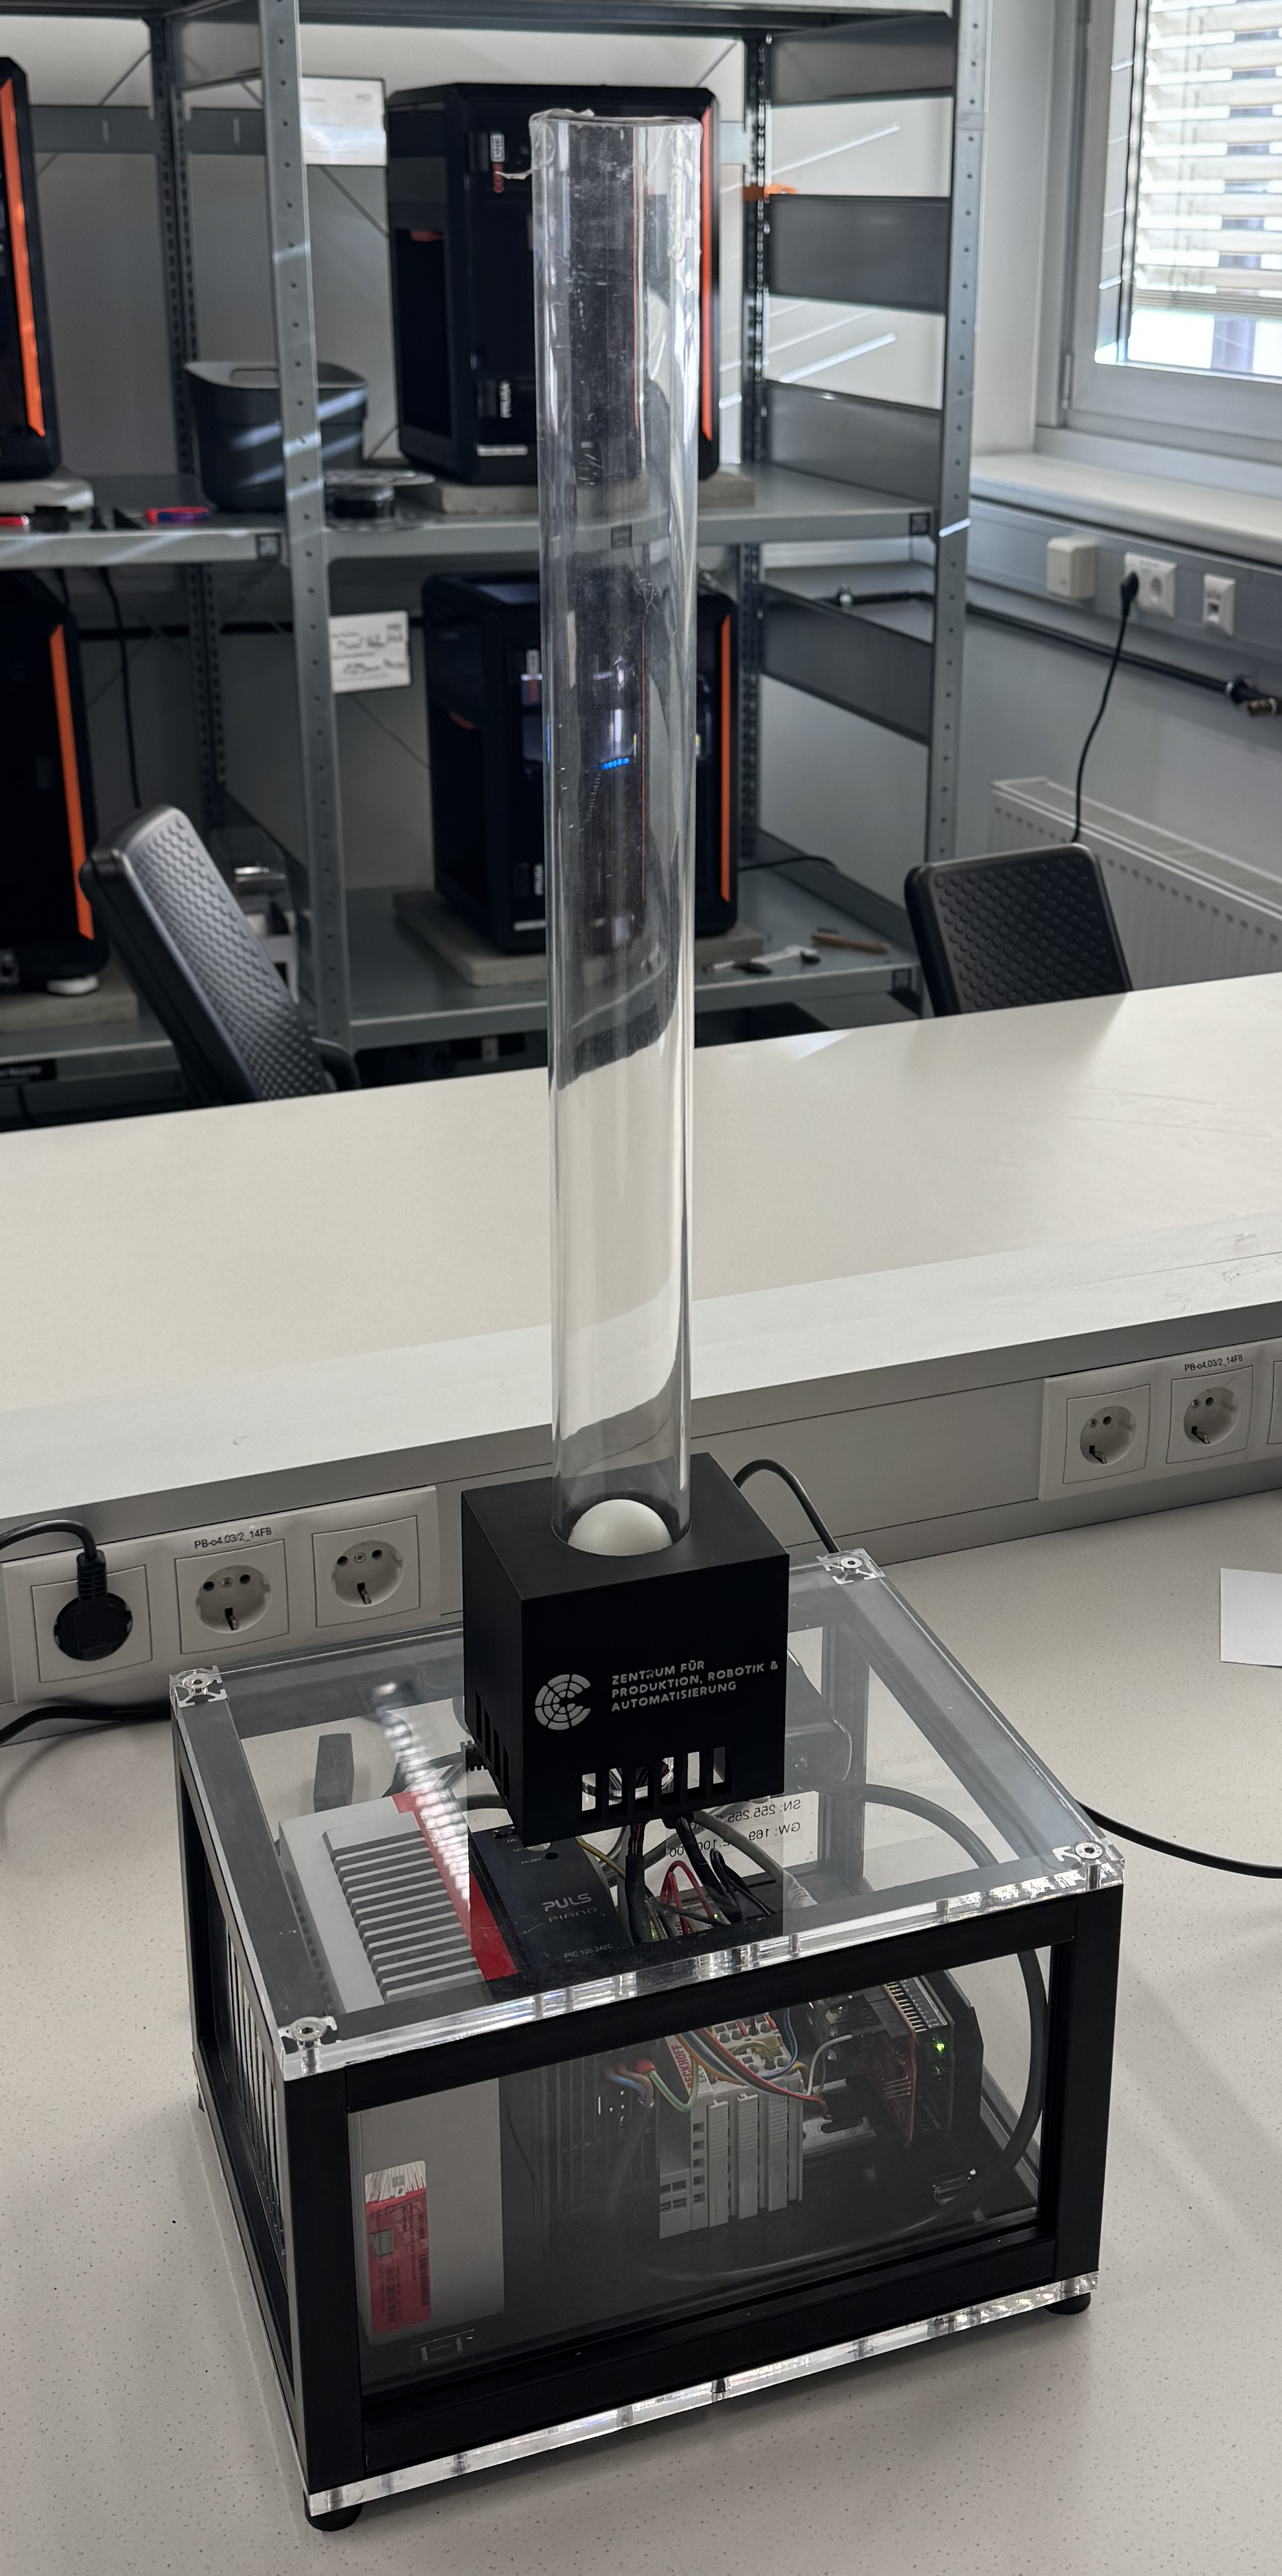
\includegraphics[width=0.225\textwidth]{img/ball_in_tube.png}
    \caption{Ball-in-Tube laboratory system}
    \label{fig:bit_system}
\end{figure}

This laboratory investigates the height control of a ping-pong ball inside a vertical tube. 
An upward air flow, generated by a fan, lifts the ball while a time-of-flight sensor, placed 
above the fan, measures its position. The task focuses on modelling the nonlinear system 
dynamics, linearising the model around a suitable operating point and designing a control 
strategy capable of regulating the ball height and enabling smooth trajectory transitions.

A simulation in MATLAB Simulink serves as the platform for analysing the system, designing the 
controller and preparing the implementation on a Beckhoff PLC. The report is structured as 
follows:
\begin{itemize} 
    \item Chapter~2 summarises the theoretical background of the system. 
    \item Chapter~3 outlines the laboratory setup and the parameter identification procedure. 
    \item Chapter~4 presents the simulation models and the controller design. 
    \item Chapter~5 discusses the results.
    \item Chapter~6 concludes the report.
\end{itemize}
